\documentclass{whutmod}
\usepackage[linesnumbered,ruled,lined]{algorithm2e}
\usepackage{diagbox}
\bibliographystyle{unsrt}
\team{10}
\membera{刘子川}
\joba{编程}
\memberb{程宇}
\jobb{建模}
\memberc{祁成}
\jobc{写作}
\hypersetup{
	colorlinks=true,
	linkcolor=black,citecolor=black
}


\newcommand{\upcite}[1]{\textsuperscript{\cite{#1}}}
%%%%%%%%%%%%%%%%%%%%%%%%%%%%%%%%%题目%%%%%%%%%%%%%%%%%%%%%%%%%%%%%%%%%%%%
\title{基于NSGA-II算法的插板式编码\\多目标优化生产调度模型}
\tihao{5} 
\everymath{\displaystyle}
\begin{document}

%	\maketitle
	\thispagestyle{empty}
%%%%%%%%%%%%%%%%%%%%%%%%%%%%%%%%%摘要%%%%%%%%%%%%%%%%%%%%%%%%%%%%%%%%%%%%
	\title{基于NSGA-II算法的插板式编码\\多目标优化生产调度模型}
	\maketitle % —— 显示标题
	\begin{abstract}
		控制高压油管的压力变化对减小燃油量偏差,提高发动机工作效率具有重要意义。本文建立了基于质量守恒定理的微分方程稳压模型,采用二分法、试探法以及自适应权重的蝙蝠算法对模型进行求解。
		\vspace{7pt}	%空格
	
		针对问题一,将规则物体三维半在线背包装载问题转化为二维排样问题,通过讨论不同包络排样方式,建立基于菱形排样的优化模型。分别讨论蜂窝包络排样、矩形包络排样和菱形排样特点并计算三种排样方式的利用率。选择理论利用率较高的菱形排样,采用贝叶斯优化最大化原材料内椭圆物料数量。实验结果表明,原材料能填充LJ1产品的数目最多为$\mathbf{36180}$个。此时每个零件产品的数量和原材料的利用率为$\mathbf{86.8345\%}$。

		%针对问题一,建立基于质量守恒定律的燃油流动模型,考察单向阀开启时间对压力稳定性的影响。综合考虑压力与弹性模量、密度之间的关系,提出燃油压力-密度微分方程模型和燃油流动方程。本文采用改进的欧拉方法对燃油压力-密度微分方程求得数值解;利用二分法求解压力分布。综合考虑平均绝对偏差等反映压力稳定程度的统计量,求得直接稳定于100MPa的开启时长为\textbf{0.2955ms} ,在2s、5s内到达并稳定于150MPa时开启时长为\textbf{0.7795ms}、\textbf{0.6734ms},10s到达并稳定于150MPa的开启时长存在多解。最后对求解结果进行灵敏度分析、误差分析。
		\vspace{7pt}	%空格
		
		针对问题二,以二维排样视角建立基于二维菱形逐层排样的最小势能堆积模型。在第一问基础上,二值化矩形排样二维空间,通过分析相叠约束和边界约束条件,使母层与子层图样镶嵌交替充满整个排样空间。表1给出了利用率最高的五种切割方案,最优方案为LJ6产品自身层叠镶嵌,材料利用率达到$\mathbf{88.0826\%}$。
		
		%针对问题二,建立基于质量守恒定律的泵-管-嘴系统动态稳压模型,将燃油进入和喷出的过程动态化处理。考虑柱塞和针阀升程的动态变动,建立喷油嘴流量方程和质量守恒方程。为提高角速度求解精度,以凸轮转动角度为固定步长,转动时间变动步长,采用试探法粗略搜索与二分法精细搜索的方法求解,求得凸轮最优转动角速度\textbf{0.0283rad/ms(转速270.382转/分钟)},并得到该角速度下高压油管的密度、压力周期性变化图。对求解结果进行误差分析与灵敏度分析,考察柱塞腔残余容积变动对高压油管压力稳态的影响。
		\vspace{7pt}	%空格
		针对问题三,设计免疫差分进化算法
		%针对问题三,对于增加一个喷油嘴的情况,改变质量守恒方程并沿用问题二的模型调整供、喷油策略,得到最优凸轮转动角速度为\textbf{0.0522rad/ms(498.726转/分钟)};对于既增加喷油嘴又增加减压阀的情况,建立基于自适应权重的蝙蝠算法的多变量优化模型,以凸轮转动角速度、减压阀开启时长和关闭时长为参数,平均绝对偏差MAD为目标,在泵-管-嘴系统动态稳压模型的基础上进行求解,得到最优参数:\textbf{角速度0.0648 rad/ms(619.109转/分钟)}、减压阀的开启时长\textbf{2.4ms}和减压阀的关闭时长\textbf{97.6ms}。
		\vspace{7pt}	%空格
		针对问题五,建立基于最小势能堆积算法的收益模型,考察总利润与利用率的相关关系。定义单产品理想收益,分析单产品方案的相对利润并得出筛除收益较小的长方体产品的结论。利用问题二的相叠约束和边界约束条件,补充体积限制的硬约束,对问题二中的方案进行优化并算出各方案对应的总利润,总利润最大的五种方案分别是$m6,m5,m18,m7,m10$,分别对应总利润$144168000,132720000,130104000,75134400,73238400$元。
		%本文的优点为:1. 采用试探法粗略搜索与二分法精细搜索结合的方法,降低了问题的求解难度。2.以凸轮转动角度为固定步长,对不同角速度按照不同精度的时间步长求解,大大提高了求解的精确度。 3.针对智能算法求解精度方面,采用改进的蝙蝠算法,使速度权重系数自适应调整,兼顾局部搜索与全局搜索能力。
		
		\keywords{
			微分方程\quad
			微分方程\quad	
			微分方程\quad
			微分方程\quad
		}
	\end{abstract}


%%%%%%%%%%%%%%%%%%%%%%%%%%%%%%%%%目录%%%%%%%%%%%%%%%%%%%%%%%%%%%%%%%%%%%%
	\thispagestyle{empty}
	\tableofcontents
	\setcounter{page}{0}  
		\thispagestyle{empty}                                             
	\newpage	%换页符
	

	
	\section{问题重述}	
		\subsection{问题背景}
	    	在大型工业产品中,如机床、轮船、飞机,常常需要很多的小零件,如螺钉、螺帽、螺栓、活塞等。在零件的生产过程中,第一步是需要依照零件产品尺寸从原材料中截取初级产品,这是零件制造的第一道工序。在这道工序中,不同的截取方案具有不同的材料利用率,而原材料的利用率(原材料截取初级产品的总体积与原材料体积之比)直接影响产品的生产成本。在市场上,零件的截面(表面)形状是多种多样的,有圆形、矩形等,零件的厚度(高度)尺寸也是大小不一的。在原材料尺寸固定的前提下,截取零件的初级产品后产生的废料最少是企业的追求。
	
	
	
		\subsection{问题概述}
		    围绕相关附件和条件要求,研究工业零件切割优化方案,依次提出以下问题:
				 
			\textbf{问题一:}用一块原料切割椭圆柱产品,通过建立数学模型给出原材料利用率最高的切割的方案。
			
			\textbf{问题二:}在一块原材料上切割椭圆柱和圆柱的六种产品,通过建立数学模型,给出利用率由高到低排序的前 5 种切割方案,即每个零件产品的数量和原材料的利用率。
			
			\textbf{问题三:}需要完成表 2 中 LJ1、LJ2、LJ3、LJ4、LJ5、LJ6 产品的生产任务,至少需要多个原材料?由于工艺的缘故,只允许至多采用 5 种切割方案,建立数学模型,给出原材料总利用率最高的至多 5 种切割方案。

			\textbf{问题四:}将问题三的产品型号拓展到 LJ1-LJ9, 需要完成表 2 中 LJ1-LJ9 产品的生产任务,同样需要多少个原材料?同样只允许至多采用 5 种切割方案,建立数学模型,给出原材料总利用率最高的至多 5 种切割方案。
				
			\textbf{问题五:}不考虑产品 LJ1-LJ9 的需求数量,给定 100 个原材料,按照表 2 中给出的利润,建立数学模型,给出总利润最大的切割方案(同样要求切割方案不超过 5 个)。
	
	\section{模型假设}
		\begin{itemize}                                             
		\item [(1)]将产品表面加工视为理想加工过程,加工后的产品与理论光滑的柱体表面质量一致,不考虑实际加工过程中产生的随机误差和系统误差。
		\item [(2)]不考虑表面粗糙度、形位公差等工艺参数的影响,将加工产品理想化为光滑的柱体。
		\item [(3)]忽略实际生产过程中铣床、刨床等加工设备与加工条件的限制,假设可以完全按照预期加工立方体原材料得到生产计划中的所有产品。
		\item [(4)]假设原材料在加工、运输等加工前的工程中没有任何损耗。
		\end{itemize}

		
	\section{符号说明}
		\begin{table}[H]
		\centering
		\setstretch{.8}   %设置表的行间距
		\setlength{\tabcolsep}{12mm}
		\begin{tabular}{cc}
			\toprule[1.5pt]
			\multicolumn{1}{m{2cm}}{\centering 符号} & \multicolumn{1}{m{10cm}}{\centering 说明} \\
			\midrule[1pt]		
			$\eta$  & 材料利用率 \\ 
			$\gamma$  & 菱形边长  \\ 
		   	$l,w,h$  & 椭圆柱长度、宽度、厚度\\ 
		   	$revenue_i$  & $LJ_i$的单产品理想收益\\ 
		   	$benefit$  & 总利润\\ 
		   	$d_{mk}$  &图案$R_i$中心点到图案$R_m$像素点的欧式距离\\ 
			\bottomrule[1.5pt]
		\end{tabular}
		\begin{tablenotes}
		\item 注:表中未说明的符号以首次出现处为准
		\end{tablenotes}
		\end{table}

	\section{问题一模型的建立与求解}
		\subsection{问题描述与分析}
		问题一要求在一块原材料上切割$LJ1$产品,求解使得原材料利用率最高的切割方式。分析问题要求及附件数据可知该问题为三维装样问题,即在一个三维长方体空间内摆入尽可能多的等径等高的椭圆柱体。为降低模型求解难度,首先将原材料沿高度切割为若干块与$LJ1$产品等高的板材,并在每块板材上进行椭圆的二维排样,其示意图如图~\ref{adffdas}~所示。如图所示,本节以此方式将三维排样问题转化为了若干个相同的二维排样问题。
			
		整理参考文献可知\upcite{1,2,3},二维等径椭圆在矩形内排样方式有矩形包络排样、正六边形包络排样与菱形包络排样等。本节分别计算并比对各排样方式理论空间利用率,之后根据附件中的材料与产品数据进行仿真排样,选择实际原材料利用率最大的排样方法作为最终排样方案,并计算其切割数量。

		鉴于矩形包络排样与正六边形包络排样的空间利用率为定值,本节直接计算其空间利用率并对其进行仿真。针对菱形包络排样,根据不同切点位置可算得不同空间利用率,本节利用贝叶斯优化求解实际原料利用率最高相切位置。
		\begin{figure}[H]
		\centering
		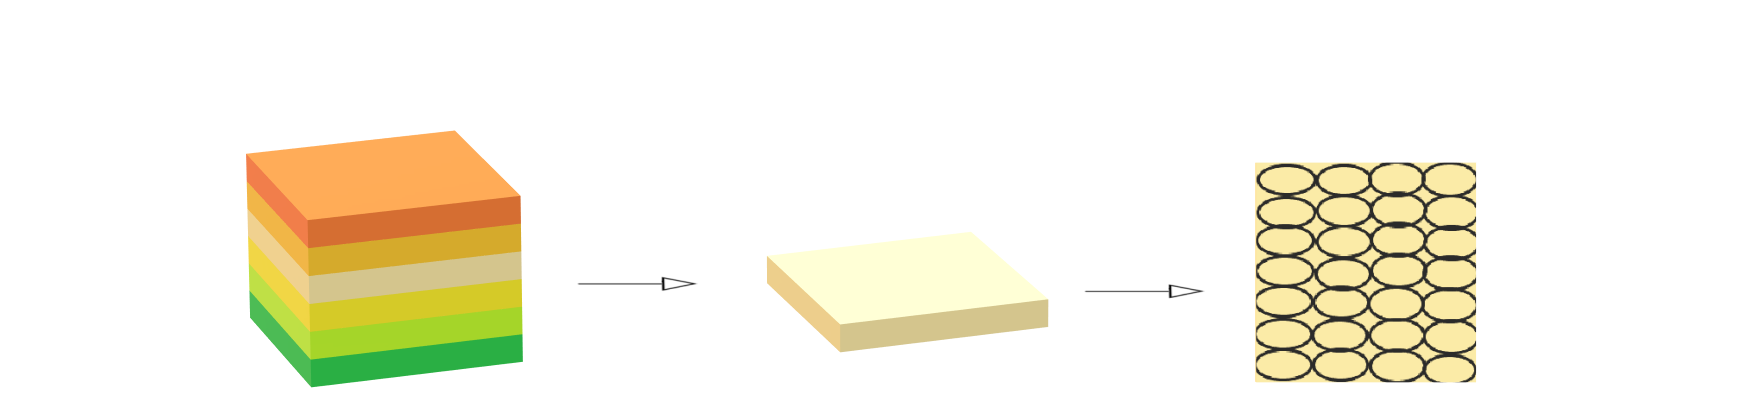
\includegraphics[width=\textwidth]{figures/11.png}
		\caption{二维展开示意图}\label{adffdas}
		\end{figure}

		\subsection{排样方式建立与模型求解}
			
		\subsubsection{包络排样方式讨论}
			\textbf{1.蜂窝包络排样:}设计一个具有二级结构的密排样基本单元,三个长轴夹角为$60^{\circ}$的两两相切的椭圆构成一个一级结构,六个一级结构围绕一个一级结构构成一个二级结构,形成蜂窝状的排样图案,如图~\ref{ccc}~所示。
			
			记蜂窝包络排样的材料利用率为$\eta_b$。建立平面直角坐标系,根据解析法求出横截距,得到三角形单元边长$\gamma_x$。从而有
			\begin{gather*}
			\eta_b=\frac{3}{2}\pi ab/\left (\frac{\sqrt{3}}{4}\gamma_x^2\right )=3\sqrt{3}\pi/31\doteq 52.7\%.
			\end{gather*}
			
			可见蜂窝包络排样理论上具有约$52.7\%$的材料利用率。
			
			
		\textbf{2.矩形包络排样:}将椭圆的最小包络矩形,即椭圆外接矩形作为排样基本单元,计算平面材料利用率。
			
			已知椭圆半长轴$a=30$、半短轴$b=20$,记矩形包络排样的材料利用率为$\eta_r$,有
			\begin{gather*}
			\eta_r=\pi ab/4ab=\pi/4\doteq 78.5\%.
			\end{gather*}
			可见矩形包络排样排布简单,具有约$78.5\%$的材料利用率。
			
			\begin{figure}[H]
				\centering
				\subfigure{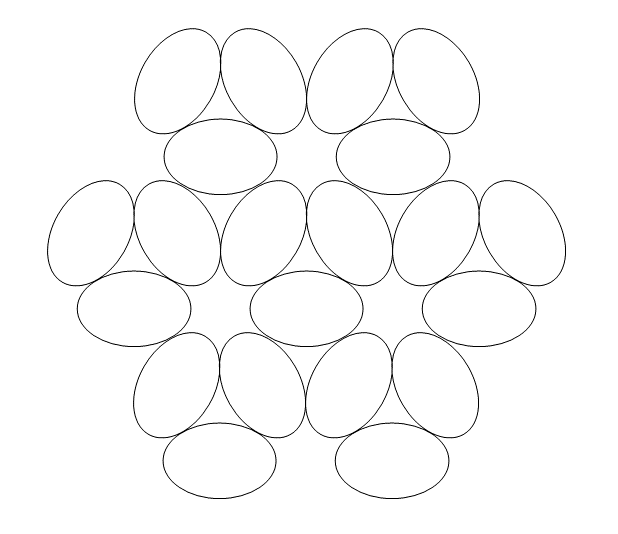
\includegraphics[height=4cm,width=5cm]{figures/bbb.png}}
				\subfigure{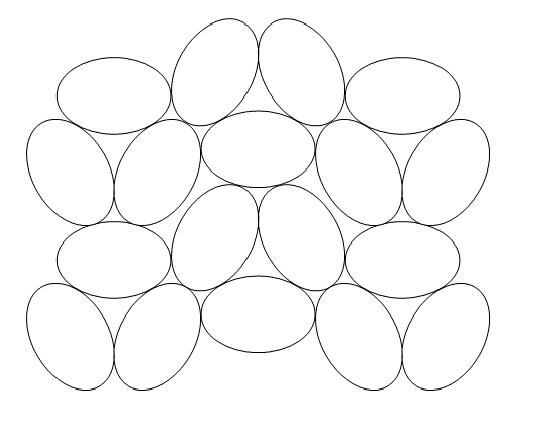
\includegraphics[height=4cm,width=5cm]{figures/ccc.png}}
				\subfigure{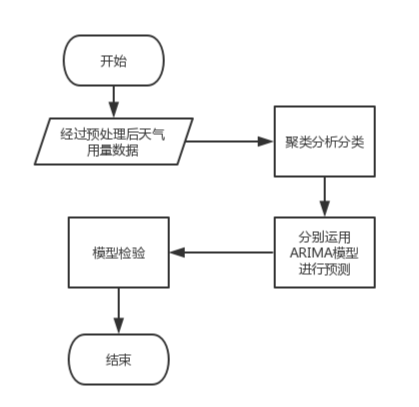
\includegraphics[height=4cm,width=5cm]{figures/aaa.png}}
				\caption{椭圆包络排样方式示意图}\label{ccc}
			\end{figure}
			
			
			\textbf{3.菱形排样:}考虑一种密排样方式,四个椭圆围绕一个中心椭圆排列,周边椭圆的中心和中部椭圆的中心仰角记作\textbf{特征角}$\theta$。记这样五个椭圆的排样形式为一个菱形排样基本模块。
			
			特征角不同,菱形排样结构有细微差异。如图~\ref{cdcc}~所示,一般情况下,中心椭圆与周围四个椭圆两两相切,理想情况下,包含中心椭圆在内的七个椭圆两两相切。
			
			一般情况下,菱形对角线可以通过参数方程中的仰角表示,记菱形排样的材料利用率为$\eta_l$,理论利用率可以表示成与椭圆仰角有关的函数
			\begin{gather*}
			\eta_l(\theta)=\pi ab/\left (4ab\sin 2\theta\right )=\pi /4\sin 2\theta.
			\end{gather*}
			
			图(a)的情况下,根据解析法求得菱形边长$\gamma =10\sqrt{31}$,对应仰角$\theta=30^{\circ}$;图(c)的情况下,根据解析法求得菱形边长$\gamma =10\sqrt{21}$,对应仰角$\theta=60^{\circ}$,即有
			\begin{gather}
			\underset{\theta \in [\frac{\pi}{6},\frac{2\pi}{3}]}{\max \eta_l(\theta)}=\pi ab/\left (\gamma ^2\sin 2\theta\right )=\pi/2\sqrt{3}\doteq 90.69\%.
			\end{gather}

			通过最大化原材料内的椭圆数目使得原料利用率最高。调整特征角大小使得原材料内排样基本模块的个数最多,构成一个单目标优化问题。在菱形排样中,如何通过调整特征角使得更多的菱形模块在原材料内而不超过原材料边缘是优化的关键。
						\begin{figure}[H]
				\centering
				\subfigure[仰角最大]{\label{fig:mdleft}{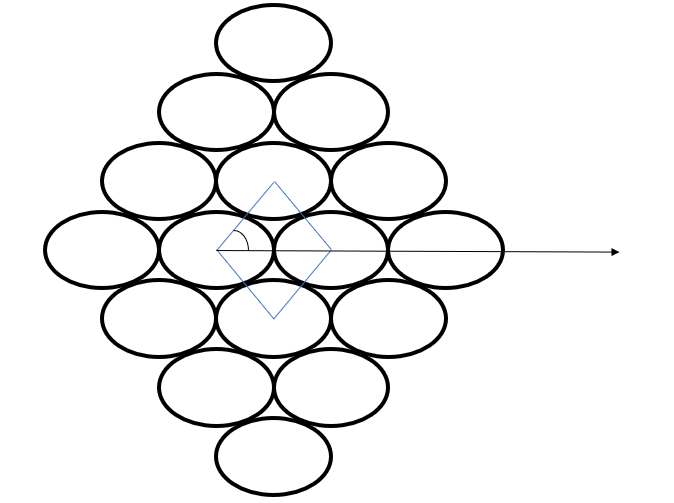
\includegraphics[width=0.3\textwidth]{figures/ddd.png}}}\hfill
				\subfigure[仰角介于中间]{\label{fig:md}{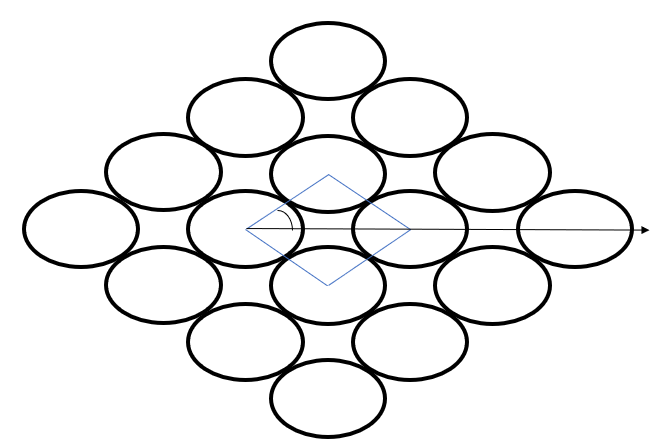
\includegraphics[width=0.3\textwidth]{figures/eee.png}}}\hfill
				\subfigure[仰角最小]{\label{fig:mdright}{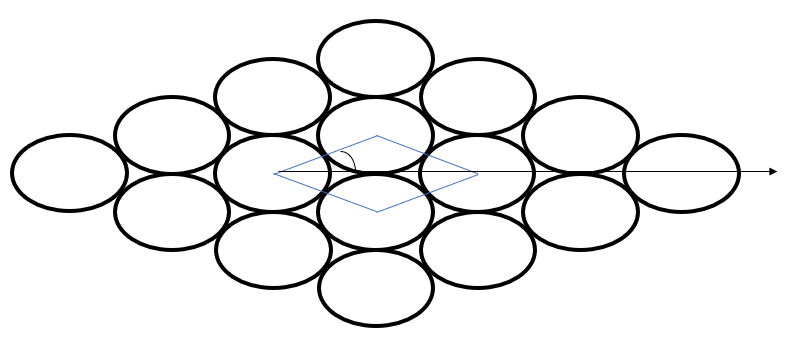
\includegraphics[width=0.3\textwidth]{figures/fff.png}}}

				\caption{椭圆菱形排样方式示意图}\label{cdcc}
			\end{figure}

			考虑到算得三种排样方式的利用率理论值不一定符合矩形区域限制,综合三种排样方式,选取理论利用率较高的菱形排样进行矩形区域原材料利用率目标优化。

			\subsubsection{目标函数及贝叶斯优化}
			菱形排样中,通过最大化原材料内的椭圆柱数目使得原料利用率最高,因此目标函数可以表示为
			\begin{align}
		&n_{ellipse}=\frac{H}{h}\times([\frac{L}{\gamma *cos\theta}]*[\frac{W}{\gamma *sin\theta}]-[\frac{W}{\gamma *sin\theta}]\div 2), 
			\\ 
			&subject\quad to: \quad \quad \quad \theta\in [\frac{\pi}{6},\frac{\pi}{3}]. \hfill
			\end{align}
			
			对于参数$l$可由对应的解析解$l=\sqrt{4ab/(bsin^2\theta +acos^2\theta )}$表示。其中$\gamma $表示菱形边长,$\theta$表示特征角,$(l,w,h),(L,W,H)$对应椭圆柱和原材料的长度、宽度和厚度,$[\cdot ]$表示向下取整函数。

			为了计算椭圆特征角的合理角度$\theta$,以使原材料内椭圆柱的个数尽可能大。根据Snoek等人的论文\upcite{8},我们采用贝叶斯优化寻找最佳椭圆特征角,其算法伪代码如下

			\begin{algorithm}[H]
			 	\caption{贝叶斯优化伪代码}  
			 	\LinesNumbered  
			 	\setstretch{1}   %设置表的行间距
			 	\KwIn{目标函数: $f$\newline
			 		超参数$\theta$搜索空间: $X$\newline
			 		采集函数: $S$
			 	}
%			 	\KwOut{frequent item sets $F$}  
			 	\textbf{Initialize} \newline
			 	 $D \leftarrow $ $InitSamples(f,x)$	\quad //初始化获取数据集\newline
			 	\For{i=1 to sizeof(D)}
			 	{
			 		$p(y|x,D)\leftarrow \textit{FitModle}(M, D)$  \quad\quad //假设模型M服从高斯分布D\newline
			 		$x_i\leftarrow argmax_{x\in X}S(x,p(y|x,D))$\newline
			 		$y_i\leftarrow f(x_i)$, $\triangleright$ Expensive step\newline
			 		 $D \leftarrow D\cup (x_i,y_i)$
			 	}
			\end{algorithm} 
		其中$f$为上述目标函数,$x_i$就是所需要寻找的角度,$S$是采样函数,$X\in [\frac{\pi}{6},\frac{\pi}{3}]$是$\theta$的搜素空间,$M$基于角度数据高斯模型\upcite{bib:8}。
        \subsection{实验结果及分析}
        实验表明,当$ 57.6^{\circ}< \theta \leqslant  60^{\circ}$时,原材料能填充 LJ1 产品的数目最多,其原材料切割方式如图~\ref{ccsdc}~所示。
        \begin{figure}[H]
        	\centering
        	\subfigure[$\theta$未经过优化的局部椭圆排列]{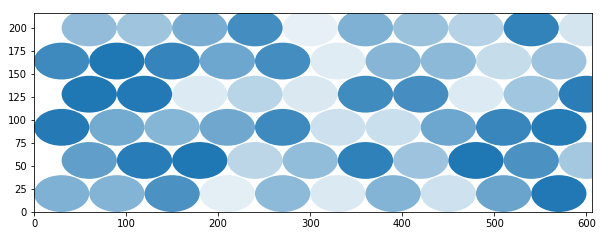
\includegraphics[width=.49\textwidth]{figures/q1.png}}
        	  \subfigure[$\theta$经过优化的局部椭圆排列]{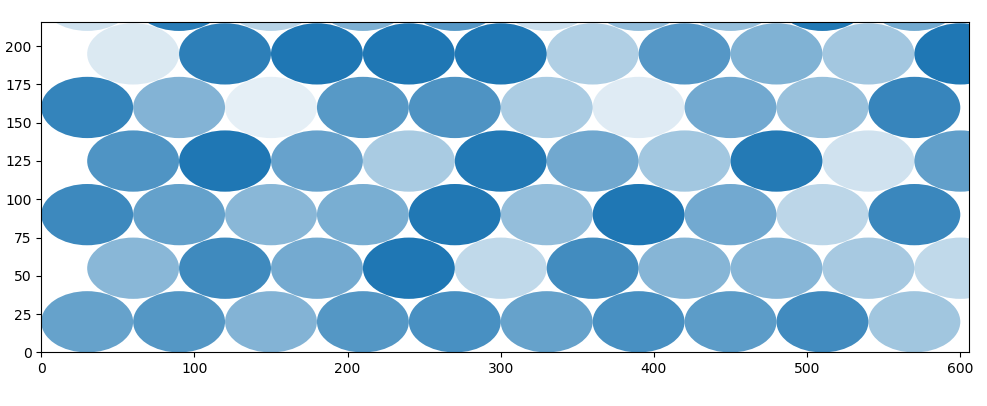
\includegraphics[width=.49\textwidth]{figures/q3.png}}
    	\subfigure[整个原材料切割示意图]{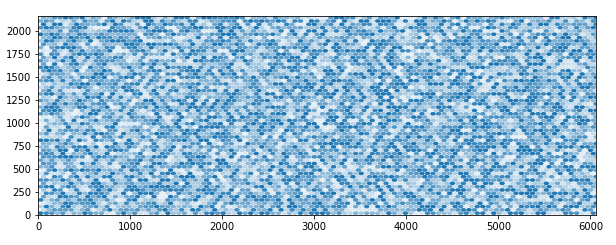
\includegraphics[width=\textwidth]{figures/q2.png}}
		\caption{原材料填充LJ1产品切割方式俯视图}\label{ccsdc}
        \end{figure}
    
    由图(a)、(b)可知,经贝叶斯优化后的$\theta$能刚好将上一排的椭圆覆盖在等比的矩形框内,及在(c)图最顶层椭圆经优化覆盖进入原材料中,使得一个原材料生产LJ1产品个数大到最大,此时一份原材料可生产产品的数量为和$36180$个,原材料的利用率为86.8345\%。

	\section{问题二模型的建立与求解}
		\subsection{问题描述与分析}
			问题二要求在一块原材料上切割LJ1、LJ2、LJ3、LJ4、LJ5、LJ6产品,给出五种原料利用率最高的切割方式。由于所有产品的厚度相等,本节沿用问题一模型,首先将原材料分割为与产品等厚的板材,将原三维装样问题转化为平面二维装样问题。分别优化求解单种产品、不同产品组合时的最优包络装样,并给出空间利用率最高的五种优化方案。问题二思维流程图如图~\ref{afsd}~所示
			
				\begin{figure}[H]
				\centering
				
\includegraphics[width=\textwidth]{figures/2liu.png}
				\caption{问题二思维流程图}\label{afsd}
			\end{figure}

		\subsection{最小势能堆积算法}
		
		问题二要求考虑六种厚度相同、二维参数不同的椭圆与圆图案排样,给出利用率最高的五种方案。问题一的解答给出,厚度相同的产品进行二维排样可以在满足排样利用率较高的前提下简化模型,且菱形排样优化使利用率提高的效果最明显。受问题一的启发,针对问题二,依然采用二维排样的模式,以层的角度进行方案比较,分析椭圆层和圆层镶嵌、圆层和圆层镶嵌两种排样方式(如图~\ref{afsd}~所示),实现两层利用率优化。之后,针对六种产品,应用两层利用率优化法进行多层组合排样,以获得利用率最高的五种排样方案。

		\begin{figure}[H]
			\centering
			\subfigure{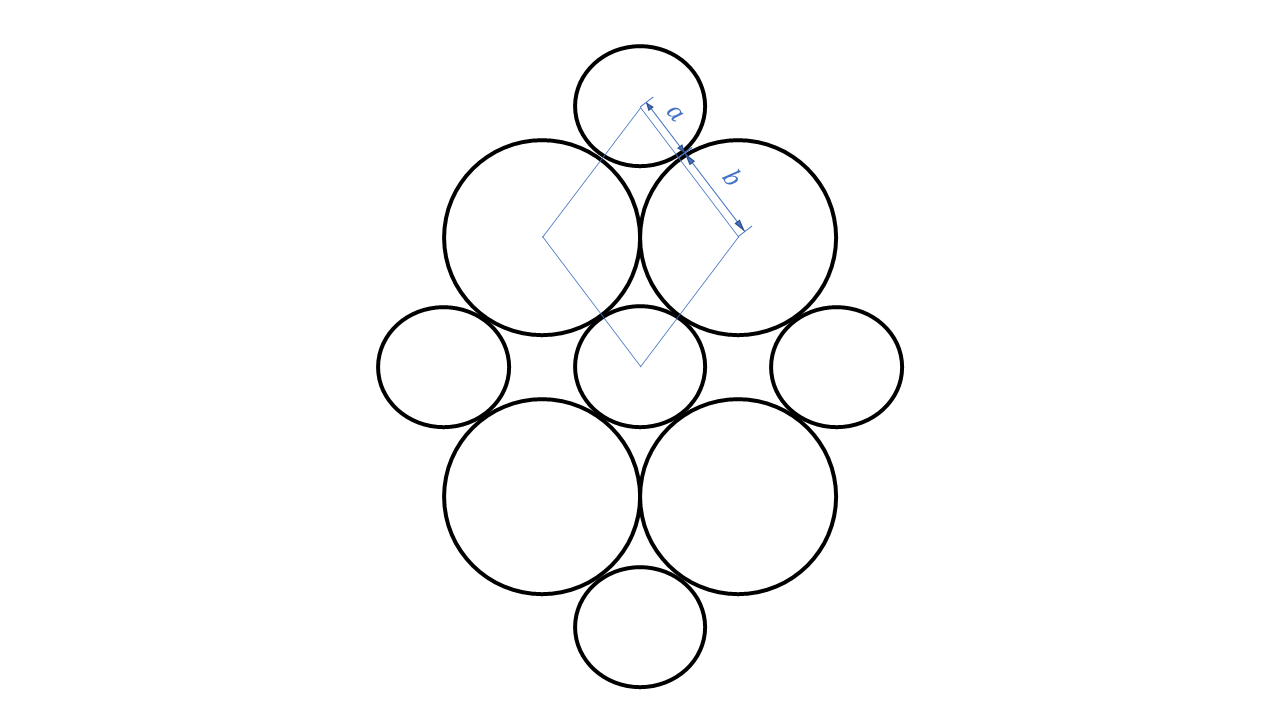
\includegraphics[width=.49\textwidth]{figures/gg1.png}}
			\subfigure{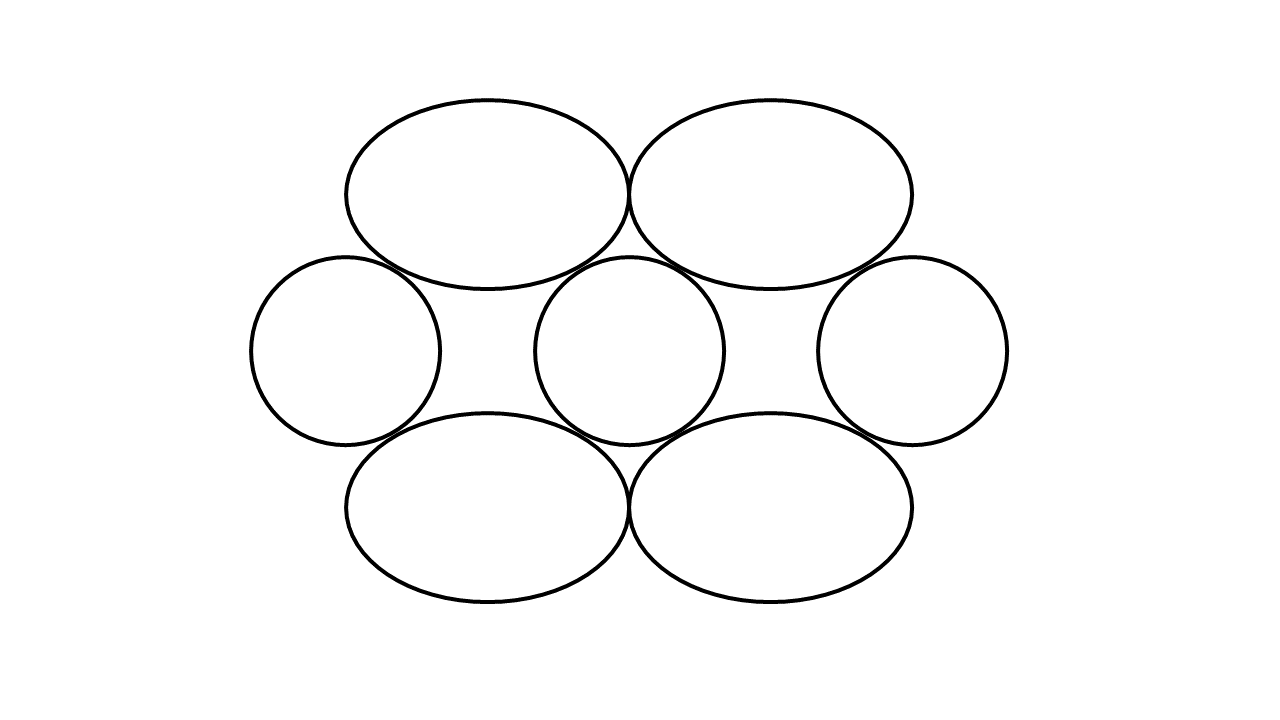
\includegraphics[width=.49\textwidth]{figures/gg2.png}}
			\caption{两种镶嵌排样方式示意图}\label{gggggg}
		\end{figure}

		圆层和圆层镶嵌的利用率可以表示为
		\begin{gather}
		\eta_{c-c}=\frac{1/2\cdot 2b\cdot 2\sqrt{a^2+2ab}}{2\theta b^2+2a^2(\pi/2-\theta)}=\frac{2b\sqrt{a^2+2ab}}{(b^2-a^2)arccos\frac{b}{a+b}+\pi/2\cdot a^2}.
		\end{gather}

		\subsection{模型的求解}
		由于LJ1-LJ6产品厚度相同,故以二维视角进行排样优化。通过二值化排样空间与排样产品,设定排样边界约束,建立最小势能堆积模型。
		
		首先考虑两种产品的排样利用率最大化。将两种产品分别排布在两层,层内所有图案相切的一层称为母层,层内图案嵌在母层空隙并且与母层图案相切的一层与称为子层。母层与子层交替排列,构成基本最小势能堆积模型。基本最小势能堆积模型中,共有四种情况,母椭圆子圆,母圆子椭圆,母子都是椭圆,母子都是圆。
		
		二值化排样空间后,排样产品覆盖区域的像素点记为1,其他像素点记为0。首先进行母层排样。当母层图案是椭圆时,保证母层内每个椭圆沿长轴相切排列,所有切点在长轴所在的共同直线上。母层排样完毕后,实现子层镶嵌。子层图案采用BL思想进行试探,以$1mm$的步长优先向排样空间左下方移动,当与母层图案有重叠时不进行移动,直到子层层内图案排样完毕,与排样空间边界不相交时循环结束。母层与子层交替排样,直至填充满整个排样空间。

        \subsection{实验结果及分析}
        由最小势能堆积算法解得在切割产品LJ1与LJ2时切割方案局部与全局对比图如下图所示
        		\begin{figure}[H]
        	\centering
        	\subfigure[局部图]{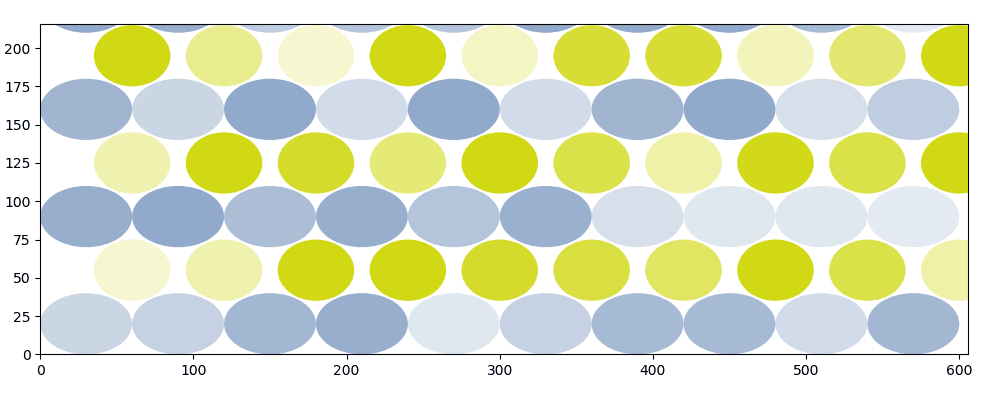
\includegraphics[width=.49\textwidth]{figures/que2/m6.png}}
        	\subfigure[全局图]{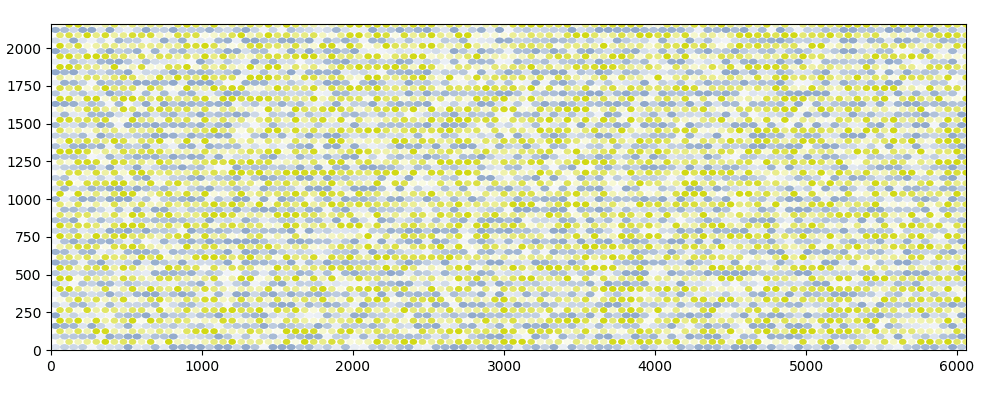
\includegraphics[width=.49\textwidth]{figures/que2/m7.png}}
        	\caption{切割方案局部与全局对比图}\label{asdfsdf}
        \end{figure}
        由图可知算法所得的排列方式为两种产品隔列排列且交错相切。将每两种产品组合排样并把每种产品单独排样可得全18种排样方式$m_1\sim m_{18}$的原材料利用率与生产产品数如下表所示
			\begin{table}[H]
			\setstretch{.5}  %设置表的行间距
			\centering		
			\caption{利用率由高到低排序的前5种切割方案}\label{zhuanssssasgzai}
			\begin{tabular}{cccc}
			\toprule[2pt]
				\multicolumn{1}{m{2cm}}{\centering 方案号}
				& \multicolumn{1}{m{3cm}}{\centering 组合方式}
				& \multicolumn{1}{m{4cm}}{\centering 工件个数}
				& \multicolumn{1}{m{4cm}}{\centering 利用率}
				\\
				\midrule[1pt]
				m1 &  LJ6、LJ6&16704、15870&88.0826\%\\ 
				m2 &  LJ4、LJ4&13104、12978&87.7423\%\\ 
				m3 &  LJ5、LJ5&14520、14388&87.4492\%\\ 
				m4 &  LJ4、LJ5&13728、13596&87.3114\%\\ 
				m5 &  LJ1、LJ1&18180、18000&86.8345\%\\ 
				m6 &  LJ2、LJ2&21780、21600&86.7624\%\\ 
				m7 &  LJ6、LJ2&18792、17940&86.696\%\\ 
				m8 &  LJ5、LJ6&15180、15042&86.5955\%\\ 
				m9 &  LJ3、LJ3&7392、6840&86.5899\%\\ 
				m10 &  LJ5、LJ2&17160、17004&85.9194\%\\ 
				m11 &  LJ4、LJ6&14352、13596&85.0461\%\\ 
				m12 &  LJ3、LJ1&10164、9576&84.8226\%\\ 
				m13 &  LJ3、LJ2&10626、10032&84.715\%\\ 
				m14 &  LJ3、LJ6&9702、9120&83.6898\%\\ 
				m15 &  LJ4、LJ2&15600、15450&83.3808\%\\ 
				m16 &  LJ3、LJ4&8778、8664&82.5534\%\\ 
				m17 &  LJ3、LJ5&9240、8664&82.4271\%\\ 
				m18 &  LJ1、LJ2&18786、18600&82.2887\%\\ 
			\bottomrule[2pt]	
			\end{tabular}
			\end{table}
		由表可知,同种产品排样的空间利用率普遍较高,即空间利用率最高的五种切割方式中有四种为单种产品排样。且产品LJ4与产品LJ5的组合排样空间利用也较高,甚至高于产品LJ2单独排样时的空间利用率。即利用率由高到低排序的前$5$种切割方案为$m1$、$m2$、$m3$、$m4$、$m5$,其原材料利用率分别为88.0826\%、87.7423\%、87.4492\%、87.3114\%与86.8345\%。四种典型的切割方案示意图如下图所示
		
		\begin{figure}[H]
			\centering
			\subfigure[切割LJ4与LJ5]{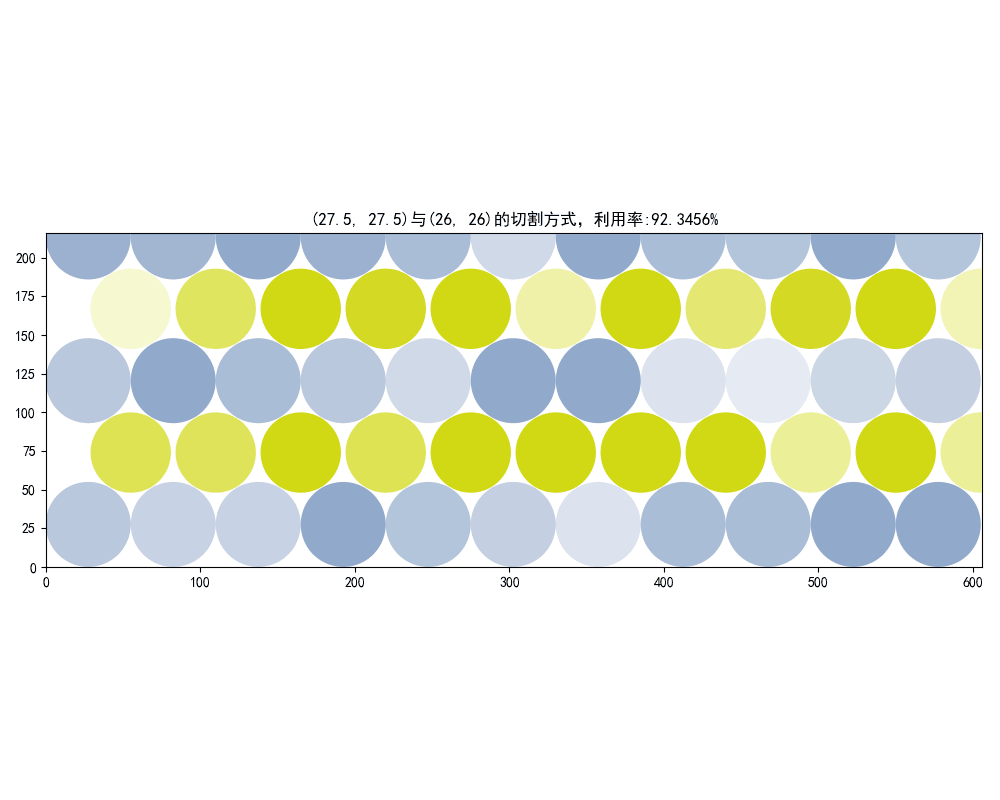
\includegraphics[width=.49\textwidth]{figures/que2/m11.JPG}}
			\subfigure[切割LJ1与LJ4]{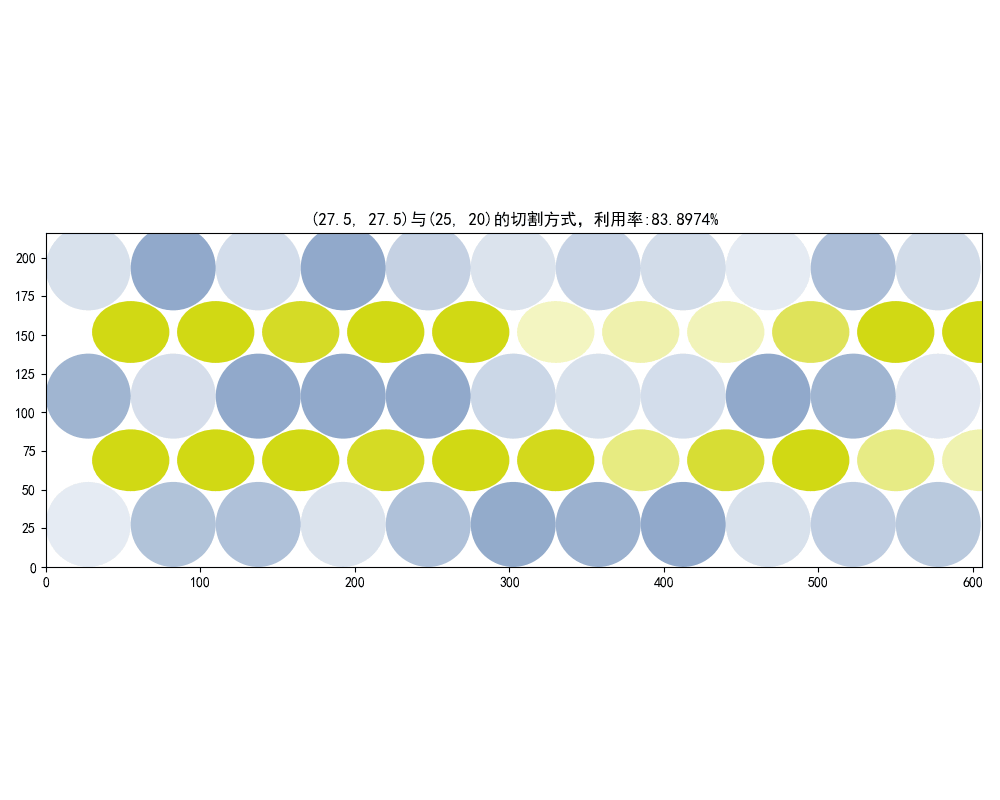
\includegraphics[width=.49\textwidth]{figures/que2/m12.JPG}}
		\subfigure[单独切割LJ2]{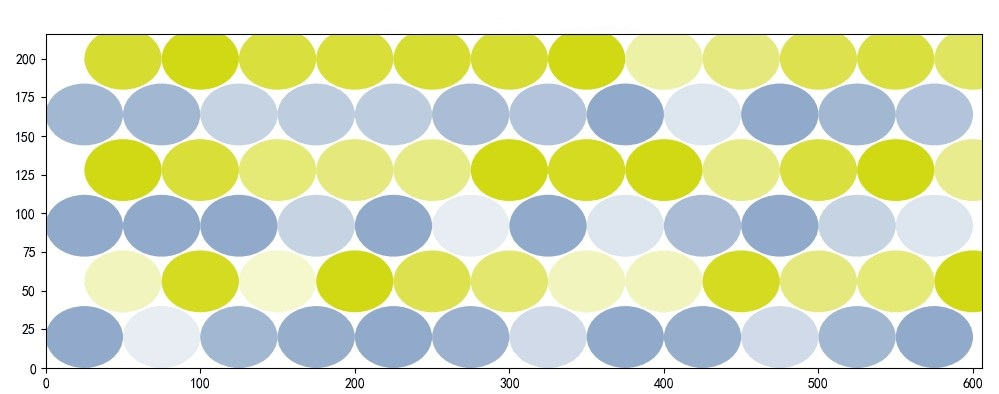
\includegraphics[width=.49\textwidth]{figures/que2/m13.JPG}}
			\subfigure[切割LJ2与LJ3]{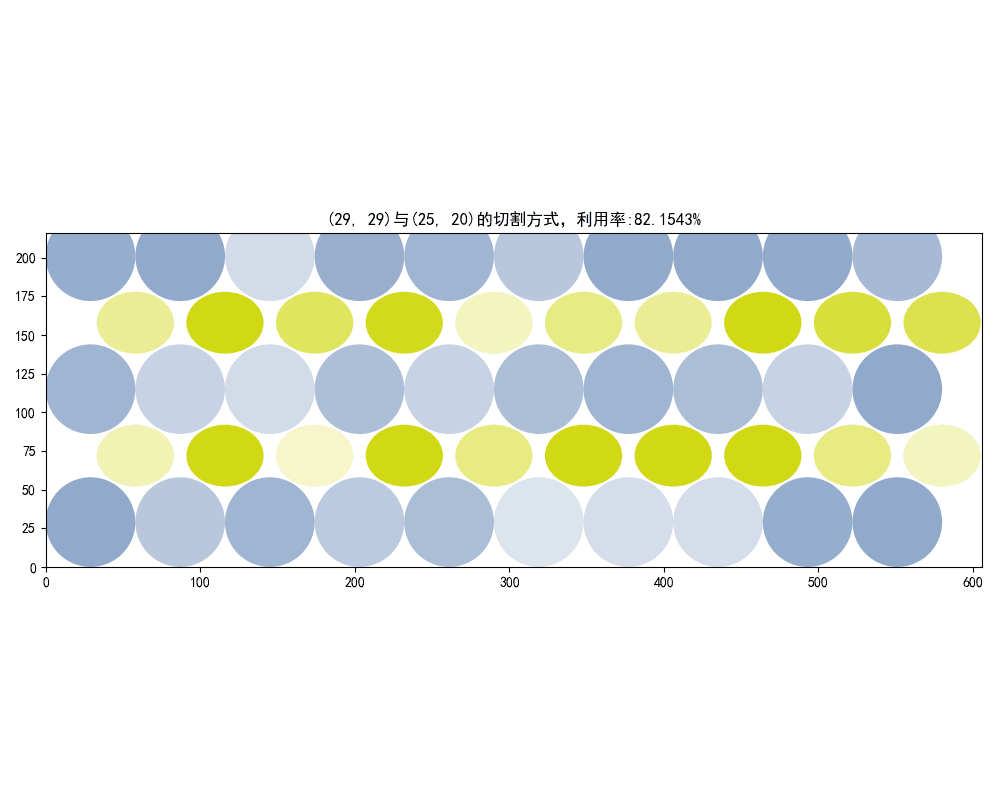
\includegraphics[width=.49\textwidth]{figures/que2/m14.JPG}}
				\caption{典型切割方案结果示意图}
		\end{figure}
%		  \begin{figure}[H]
%			\centering
%			\subfigure{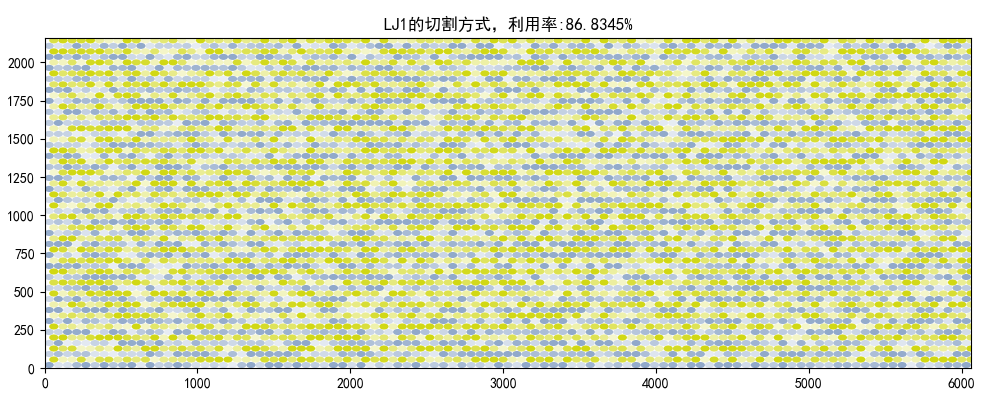
\includegraphics[width=\textwidth]{figures/que2/m5.png}}
%			\caption{利用率由高到低排序的前5种切割方案}\label{ccsdaddc}
%		\end{figure}
%
%		  \begin{figure}[H]
%			\centering
%			\subfigure{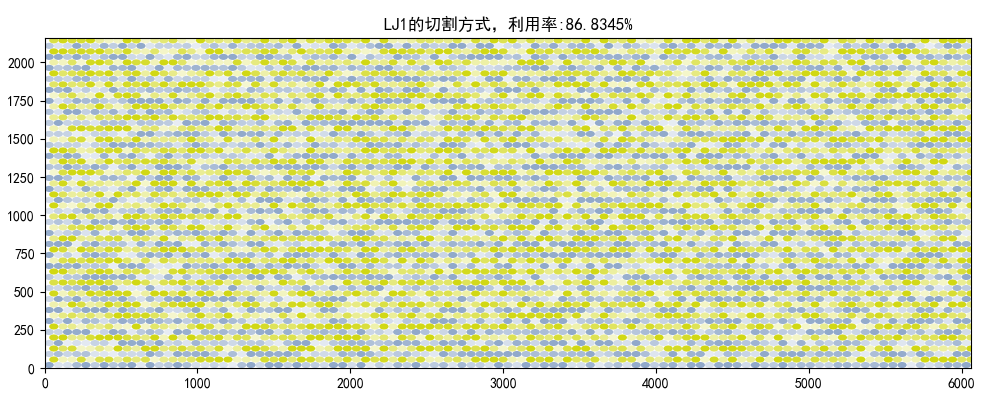
\includegraphics[width=\textwidth]{figures/que2/m5.png}}
%			\caption{利用率由高到低排序的前 5 种切割方案}\label{ccsdaddc}
%		\end{figure}
  
    \section{问题三模型的建立与求解}
    	\subsection{问题描述与分析}
        问题三要求使用最少的原材料完成中 LJ1、LJ2、LJ3、LJ4、LJ5、LJ6 产品的生产任务。鉴于所有产品的厚度仍然相同,我们仍沿用之前模型,首先将原材料二维化,之后将原材料分为不同区域,在每个区域中执行不同的模型二中解得的切割方案,即可得到一种原材料切割方案。在确定了所有切割方案后,优化各个切割方案执行次数以求解使用原材料最小的总切割方案,即问题可被转化为高维度线性规划问题。
        
        针对整体优化模型,本文设计免疫差分进化算法,并嵌入线性规划,优化求解最节省原材料的切割方案。首先各切割方案的区域分配比例作为算法决策变量,将这些切割方案带入线性规划模型,再以线性规划结果作为适应度函数,循环迭代以寻找最优切割方案。问题三思维流程图如图~\ref{asdasf}~所示	
        \begin{figure}[H]
        	\centering
        	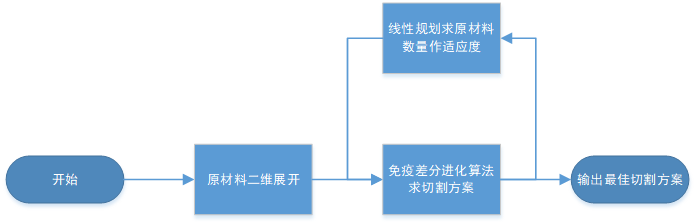
\includegraphics[width=.8\textwidth]{figures/3liu.png}
        	\caption{问题二思维流程图}\label{asdasf}
        \end{figure}
    
    		\subsection{切割比例分配模型}
    		沿用问题一、二模型将原材料切割为与产品等厚的板材后,我们将每个板材分为若干区域$\left \{ S_i \right \}$,其中区域$S_i$将使用模型二中的切割方式$m_i$进行切割操作,分割示意图如图~\ref{inoni}~所示。定义$S_i$占用的板材面积比例为$p_i$,即可将该分割方式定义为决策向量如下
    	\begin{gather*}
    	P=[p_1,p_2,\cdots,p_n] ,
    	\end{gather*}
    	其中$0\leqslant p_i\leqslant 1$且$\sum_{i=1}^n p_i=1$。即五种切割方案可表示为决策矩阵如下
    	\begin{gather}
    D=\begin{bmatrix}P_1
    \\ P_2
    \\ P_3
    \\ P_4
    \\ P_5
    \end{bmatrix}=\begin{bmatrix}
    p_{1,1}&  p_{1,2} & \cdots &p_{1,n} \\
    p_{2,1}&  p_{2,2} & \cdots &p_{2,n} \\
    p_{3,1}&  p_{3,2} & \cdots &p_{3,n} \\
    p_{4,1}&  p_{4,2} & \cdots &p_{4,n} \\
    p_{5,1}&  p_{5,2} & \cdots &p_{5,n} 
    \end{bmatrix}.
    	\end{gather}
    	  \begin{figure}[H]
    		\centering
    		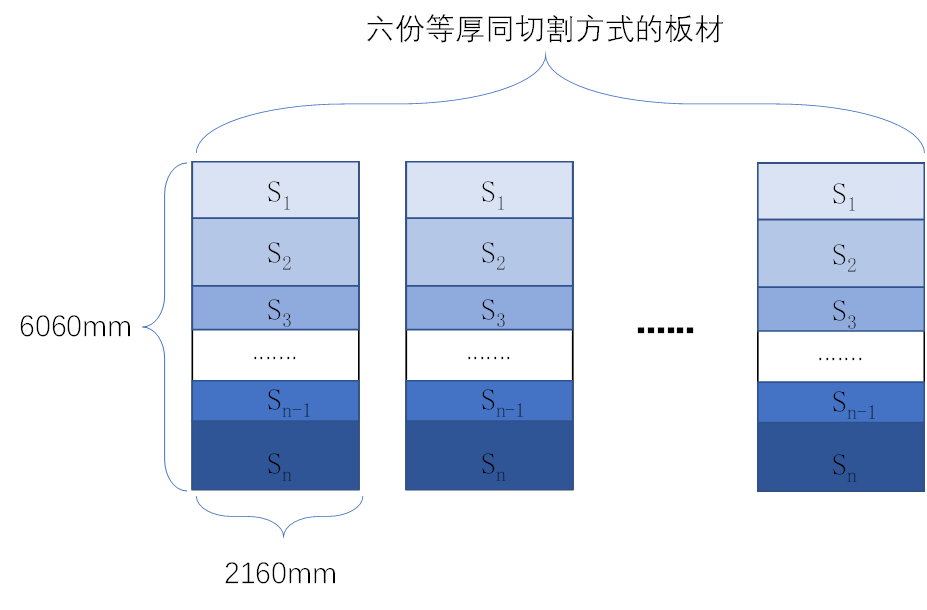
\includegraphics[width=.7\textwidth]{figures/3.png}
    		\caption{区域分割示意图}\label{inoni}
    	\end{figure}
  由决策矩阵$D$即可求解出各个方案中的分割区域$\left \{ S_i \right \}$,之后即可利用问题一、二中的贝叶斯优化算法解得每种分割方式可生产各种产品的数量,如当一块原材料使用分割方式$P_i$后可生产产品数量可表示为
  	\begin{gather*}
  W_i=[w_{i,1},w_{i,2},w_{i,3},w_{i,4},w_{i,5},w_{i,6}],  
  \end{gather*}
    其中$w_{i,1} \sim w_{i,6}$分别表示使用分割方案$P_i$时可生产得的产品LJ1、LJ2、LJ3、LJ4、LJ5、LJ6的数量。若使用切割方式$P_i$的原材料数量为$x_i$,则对于$5$种切割方式$P_1 \sim P_5$有约束函数如下 
    	\begin{gather}
  \left\{\begin{matrix}w_{1,1} x_1+w_{2,1} x_2+w_{3,1} x_3+w_{4,1} x_4+w_{5,1} x_5\geqslant N_1
  \\ w_{1,2} x_1+w_{2,2} x_2+w_{3,2} x_3+w_{4,2} x_4+w_{5,2} x_5\geqslant N_2
  \\ w_{1,3} x_1+w_{2,3} x_2+w_{3,3} x_3+w_{4,3} x_4+w_{5,3} x_5\geqslant N_3
  \\ w_{1,4} x_1+w_{2,4} x_2+w_{3,4} x_3+w_{4,4} x_4+w_{5,4} x_5\geqslant N_4
  \\ w_{1,5} x_1+w_{2,5} x_2+w_{3,5} x_3+w_{4,5} x_4+w_{5,5} x_5\geqslant N_5
  \\ w_{1,6} x_1+w_{2,6} x_2+w_{3,6} x_3+w_{4,6} x_4+w_{5,6} x_5\geqslant N_6
  \\x_1,x_2,x_3,x_4,x_5\geqslant 0
  \end{matrix}\right.,
    \end{gather}
    其中$N_1\sim N_6$分别表示产品LJ1、LJ2、LJ3、LJ4、LJ5、LJ6的要求生产数量,即生产各零件数量需不小于其要求的生产数量。再此情况下使得使用的总原材料数量最小,即
    	\begin{gather}
   min\sum_{i=1}^5x_i
    \end{gather}
    即此时问题可被转化为整数规划问题如下
    \begin{gather}
    min\sum_{i=1}^5x_i\\
     \left\{\begin{matrix}
    x_1,x_2,x_3,x_4,x_5\geqslant 0
    \\x_1,x_2,x_3,x_4,x_5\in Z
    \\\forall i=1,2,\cdots5 :w_{1,i} x_1+w_{2,i} x_2+w_{3,i} x_3+w_{4,i} x_4+w_{5,i} x_5\geqslant N_i
    \end{matrix}\right..
    \end{gather}
    \subsection{免疫差分进化算法}
     \subsubsection{浮点数编码}
      首先将决策矩阵$D=[P_1,P_2,P_3,P_4,P_5]^T$转化为浮点数编码以方便后续运算,设计浮点数向量$C_i=[c_{i,1},c_{i,2},\cdots,c_{i,n}](0<c_{i,j}<1,j\in[1,n])$来表示$P_i=[p_{i,1},p_{i,2},\cdots,p_{i,n}]$,即$C_i$与$P_i$的编码转化方式为
      \begin{gather*}
      p_{i,j}=\frac{c_{i,j}}{\sum _{j=1}^n c_{i,j}}
      \end{gather*}
      即决策矩阵$D=[P_1,P_2,P_3,P_4,P_5]^T$可以替换为浮点数染色体$S=[C_1,C_2,C_3,C_4,C_5]$。设定种群规模为$p$,即在种群初始化时使用蒙特卡洛法生成$p$个初始解,即使$c_{i,j}=rand(0,1)$。
      \subsubsection{适应度计算}
      根据浮点数染色体$S=[C_1,C_2,C_3,C_4,C_5]$可将每块原材料分割为不同方案$\left \{ m_i \right \}$的切割区域,即可求得方案各对应的产品生产数量 $W=[w_{1},w_{2},w_{3},w_{4},w_{5},w_{6}]$作为整数规划参数。放松整数优化限制$x_1,x_2,x_3,x_4,x_5\in Z$即使得$x_i$可取为浮点数变量,即可将原整数规划模型转为线性规划模型,求解该参数环境下的规划目标$\sum_{i=1}^5x_i$作为染色体$S=[C_1,C_2,C_3,C_4,C_5]$的适应度。即
       \begin{gather*}
      f(S)=min\sum_{i=1}^5x_i.
      \end{gather*}
      \subsubsection{交叉变异}
    在第$g$次迭代中,生成变异个体$H_i$,从种群中随机选取三个染色体$S_{p1}$,$S_{p2}$和$S_{p3}$,且$p_1\neq p_2\neq p_3\neq i$,生成的变异向量为
    \begin{gather*}
    H_i(g)=S_{p1}+F(g)\cdot (S_{p2}-X_{p3}),
    \end{gather*}
    $F(g)\in (0,1)$是每一代中的放缩因子,其服从柯西分部。对第$g$代种群中第$i$个体进行交叉操作,生成交叉个体$V_i(g)$,具体表达式如下:
    \begin{gather*}
    v_{i,j}=\left\{\begin{matrix}h_{i,j}(g),rand(0,1)\leq cr_{i},
    \\ c_{i,j}(g),rand(0,1)>cr_{i},
    \end{matrix}\right.
    \end{gather*}
    其中$cr_{i}\in[cr_{l},cr_{u}]$是个体$i$的交叉概率,参数$cr_{i}$将进行自适应调整,具体表达式如下:
    \begin{gather*}
    cr_{i}=\left\{\begin{matrix}cr_{l}+(cr_{u}-cr_{l})\frac{f(s_{i})-f_{min}}{f_{max}-f_{min}} , f_{i}>\overline{f},
    \\ cr_{l},f(s_{i})\leqslant  \overline{f}.
    \end{matrix}\right.
    \end{gather*}
    其中$0.1\leqslant cr_{u}<cr_{l}\leqslant 0.6$表示交叉概率的上下限,$f_{max}$、$f_{min}$与$\overline{f}$分别表示第$g$代所有解的适应度函数的最大值、最小值与平均值。
      \subsubsection{免疫选择}
    混合第$g$代的交叉个体$\left \{ V\right \}$与原始个体$\left \{ S \right \}$,得到待选组$\left \{ S '\right \}$如下
    \begin{gather*}
    S_i '=\left\{\begin{matrix}  S_i ,i\leqslant p,
    \\  V_{i-p},i>p.
    \end{matrix}\right.
    \end{gather*}
    个体 $S_a'$和$S_b '$的亲和度$M_{a,b}$可表示为
    \begin{gather*}
    M_{a,b}=|S_a'-S_b '|,
    \end{gather*}
    $M_{a,b}$表示$S_a'$和$S_b '$间的欧式距离。定义个体$S_i'$的抗体浓度为$Q_{i}$,即
    \begin{gather*}
    Q_{i}=\frac{1}{2p}\sum _{j=1}^{2p} N_{i,j},\\
    N_{i,j}=\left\{\begin{matrix}1,S_{i,j}< \mu,
    \\ 0,S_{i,j}\geqslant \mu  ,
    \end{matrix}\right.
    \end{gather*}
    $\mu(\mu\in[0,1])$为相似度阈值,即当个体$i$和$j$的亲和度$M_{i,j}<\mu$时认为个体$i$和$j$为相似个体。$Q_{i}$即为$\left \{ S'\right \}$中$S_i'$的相似个体所占比例,$Q_{i}$越大即表示$S_i '$周围区域的解密度越大。本文优先将目标函数$f$值最优的前$\sigma$个解放入下一代个体$\left \{ X\right \}$中以防止最优解丢失。再计算剩余个体的复合适应度函数如下
    \begin{gather*}
    F(S_i ')=\frac{f(S_i')-f_{min}}{f_{max}-f_{min}}+Q_{i}
    \end{gather*}
    即选取复合适应度函数$F$最小的剩余$p-\sigma$个个体放入下一代个体$\left \{ S\right \}$中。重复迭代上述算法$G$次后终止算法并输出最优参数集$S_{best}$。算法流程图如图~\ref{jndfg}~所示
    \begin{figure}[H]
    \centering
   	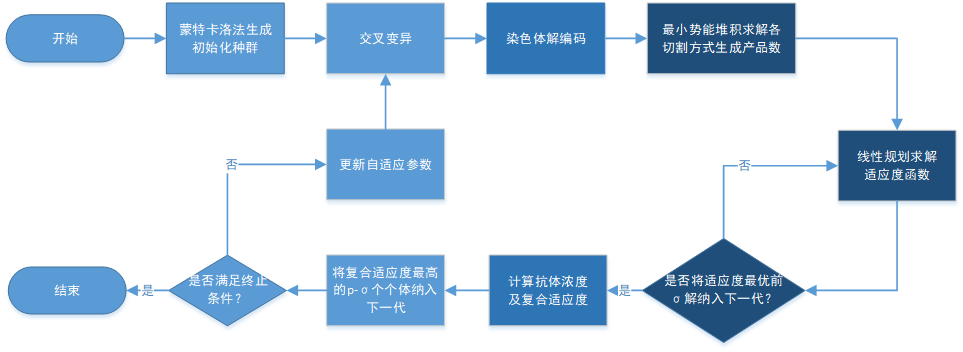
\includegraphics[width=\textwidth]{figures/chafen.png}
   	\caption{免疫差分进化算法流程图}\label{jndfg}
    \end{figure}
    \subsection{结果分析}
    通过免疫差分进化算法优化计算最佳切割方式,所得收敛结果如图~\ref{asdmsd}~(a)所示,即算法大约在第$65$次迭时代达到收敛,解得最小原材料使用量为$473$份原材料。
    	\begin{figure}[H]
    	\centering
    	\subfigure[算法收敛结果]{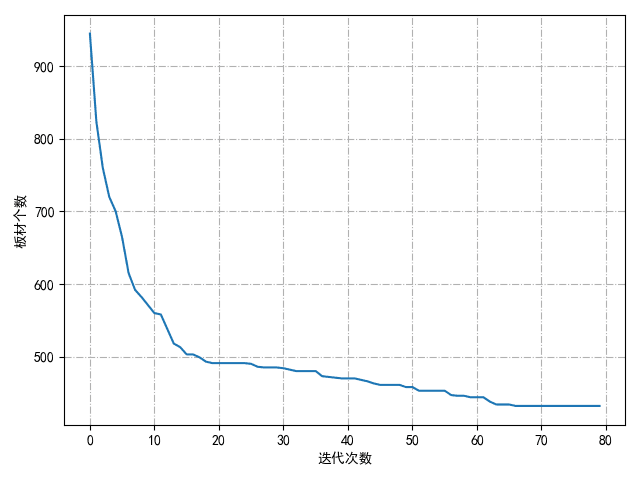
\includegraphics[width=.49\textwidth]{figures/d2.png}}\label{asdmd}
    	\subfigure[各方案生产产品数]{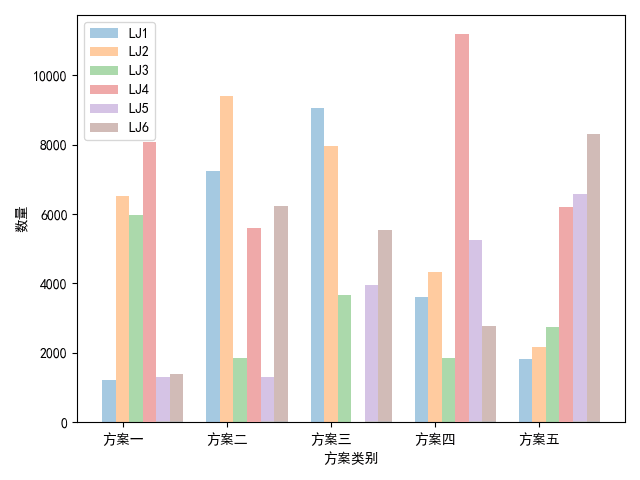
\includegraphics[width=.49\textwidth]{figures/f2.png}}
    	\caption{免疫差分进化算法结果图}\label{asdmsd}
    \end{figure}
    最优方案中各方案生产各类产品数如图~\ref{asdmsd}~(b)所示,其中方案一、方案二、方案三、方案四、方案五的生产细明如表
    \begin{table}[H]
    	\setstretch{.5}  %设置表的行间距
    	\centering		
    	\caption{问题三生产细明}\label{zhuanssssasgzai}
    	\begin{tabular}{cccccccc}
    		\toprule[2pt]
    		\multicolumn{1}{m{2cm}}{\centering }
    		& \multicolumn{1}{m{2cm}}{\centering 原材料数}
    		& \multicolumn{1}{m{1cm}}{\centering LJ1}
    		& \multicolumn{1}{m{1cm}}{\centering LJ2}
    		& \multicolumn{1}{m{1cm}}{\centering LJ3}
    		& \multicolumn{1}{m{1cm}}{\centering LJ4}
    		& \multicolumn{1}{m{1cm}}{\centering LJ5}
    		& \multicolumn{1}{m{1cm}}{\centering LJ6}
    		\\
    		\midrule[1pt]
    	    方案一 & 12 &  14472     &  78132  &     71640   &    96912 &      15768    &   10632\\ 
    		方案二 & 0&  0   &  0 &      0 &     0 &     0    &       0\\ 
    		方案三 & 29& 262392   &   230753   &   106488    &       0   &   114318    &  160776\\ 
    		方案四&  113&   408834 &     490307 &     207468 &    1263114&      593928    &  313236\\ 
    		方案五 & 332 & 601584   &   754304  &    914328 &    2061720&     1816040 &    1997312\\ 
    		  总计 &487 &  1287282  &   1553496  &   1199924   &  3421746   &  2540054   &  2481956\\ 
    		生产要求 &$\backslash$ & 1272000&1521000 &1161000 & 3229500&2434500 & 2421000\\ 
    		多余生产 &$\backslash$ &  15282    &   32496   &   38924     & 192246    &  105554    &   60956\\
    		冗余比例 &$\backslash$&  1.20\%   & 2.14\% &   3.35\%   & 4.95\% &  4.34\%   & 2.52\% \\ 
    		\bottomrule[2pt]	
    	\end{tabular}
    \end{table}
   由表可知,优化结果只使用$4$种分割方案,即切割方案二生产数为$0$,且所有工件的生产冗余比例皆小于5\%,在可容忍范围内。
  	\section{问题四模型的建立与求解}
  	\subsection{问题描述与分析}
  		问题四在问题三的基础上将产品扩充至LJ1$\sim$LJ9,求解需要原材料的最小数量。由于产品LJ7、LJ8和LJ9是与LJ1$\sim$LJ6厚度不同的长方体,难以沿用问题一、二、三模型使其与LJ1-LJ6在同一二维平面上进行排样。为降低问题复杂度,单独使用一种切割方式生产产品LJ7、LJ8、LJ9,即将该部分问题转化为长方体三维装箱问题,本节采用启发式算法对该三维装箱问题进行优化求解。其余四种切割方式沿用问题三模型与算法求解生产产品LJ1-LJ6所需的最小原材料数量。问题四思维流程图如图~\ref{dfasfd}~所示
  	\begin{figure}[H]
  		\centering
  		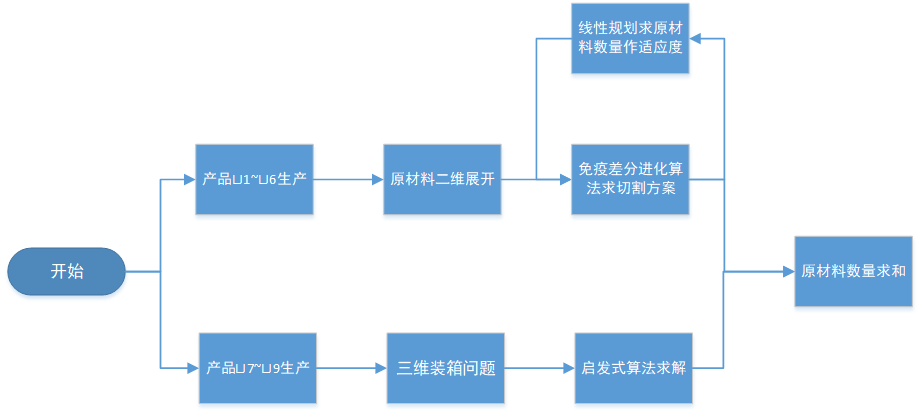
\includegraphics[width=.7\textwidth]{figures/4liu.png}
  		\caption{问题四流程图}\label{dfasfd}
  	\end{figure}
  	
  	\subsection{三维装箱模型的建立}
  	若以一种切割方式完成LJ7、LJ8、LJ9的生产,为使得使用原材料利用率尽可能高,则需使得该切割方式生产LJ7、LJ8、LJ9的数量比$w_7:w_8:w_9$尽可能接近LJ7、LJ8、LJ9的需求量之比$N_7:N_8:N_9$。在$w_7$,$w_8$,$w_9$值确定后,将原材料视为矩形容器,产品LJ7、LJ8与LJ9视为待装入箱子,即可将LJ7、LJ8、LJ9的生产问题转化为三维装箱问题,其示意图如图~\ref{sdaasd}~所示。装箱过程须满足三个著名约束\upcite{8}如下
  	\begin{itemize}
  			\item[C1:]方向性约束,即箱子的装载具有方向性约束,也就是说,每个箱子只能按照其给定的放置姿态进行放置。
  			\item[C2:]稳定性约束,即每个被装载箱子必须得到容器底部或者其他已装载箱子的支撑。
  		\item[C3:]完全切割约束,即要求在最终的装填状态中,已放入箱子的集合可以由多个竖直的平面分割成多个子空间,并且每个子空间又可以被多个水平的平面分割成更小的子空间。
  	\end{itemize}
    \begin{figure}[H]
  	\centering
  	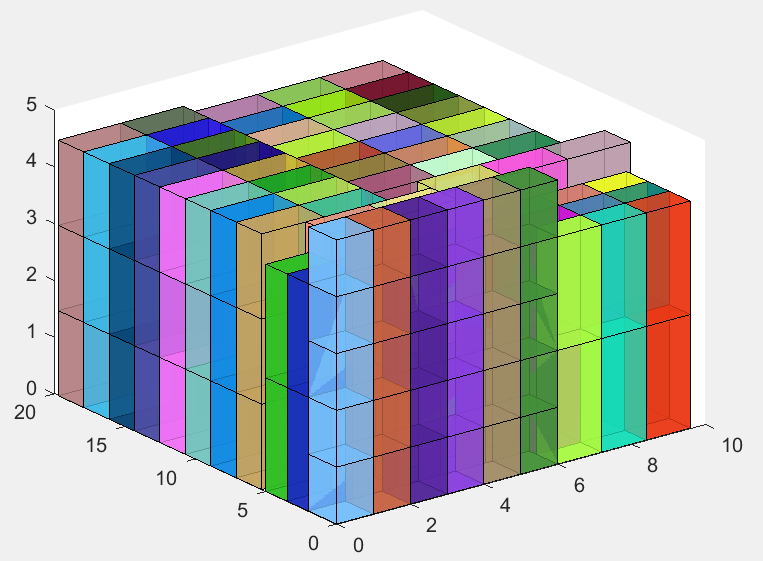
\includegraphics[width=.6\textwidth]{figures/ac.png}
  	\caption{三维装箱示意图}\label{sdaasd}
  \end{figure}
  	\subsection{3D-RSO算法}
  	放置规则的作用是能够为当前箱子选择一个合适
  	的放置空间和放置方式。基于剩余空间最优化的基本
  	求解策略,具体放置规则如下:
  		\begin{itemize}
  		\item[1:]	首先认为箱子的底面
  		积与其放置空间的底面积越接近,则越需要被优先匹配
  		布置。这是因为一方面将较大的可放置子空间空出,以
  		便于增加后续箱子的放置概率,另一方面也有利于减少
  		箱子放置后所产生的可能浪费剩余空间。
  		\item[2:]	当存在多
  		个与箱子底面积大小类似的放置空间时,优先选择能生
  		成较大剩余子空间的放置方式。
  	\end{itemize}
   根据放置规则,定义评价公式如下
   \begin{gather*}
  f(b_i,S_j)=-(l(S_j)-l(b_i)+\alpha )\cdot(w(S_j)-w(b_i)+\alpha ),
   \end{gather*}
  其中$l(S_j)$、$w(S_j)$ 分别表示放置空间的长和宽,$l(b_i)$和
  $w(b_i)$ 表示箱子放入时底面积的长和宽,$\alpha$ 是被赋值为
  0.1的修正参数,$f (b_i ,S_j)$ 的值越大越好。$3D-RSO$算法伪代码如下所示
  
 \begin{algorithm}[H]
 	\caption{3D-RSO伪代码}  
 	\LinesNumbered  
 	\setstretch{1.1}   %设置表的行间距
 	%			 	\KwOut{frequent item sets $F$}  
 	\textbf{Initialize} \newline
 	将所有箱子按照其可能产生的最大底面积降序排列,以
 	此形成集合 $BR$\newline
 	\While{  $BR\neq \varnothing$ }{
 	选择 $BR$ 中的第一个箱子作为当前箱子,并计算其在
 	所有可放置状态下的评价度$f(b_i,S_j)$,形成集合$SF$ \newline
 	\eIf{ $SF\neq \varnothing$}{
 		以评价度最高的状态对当前箱子进行放置\newline
 	   分割空间\newline
 	   删除$BR$中的$b_i$
 }
 	{删除$BR$中的$b_i$}
 	更新$BR$\newline
 	更新$SF$
 }
 \end{algorithm} 
 使用$3D-RSO$算法求解LJ7、LJ8、LJ9的生产切割方式后,沿用问题三中模型与算法,优化求解使用原材料最少的$4$种切割方式以生产产品$LJ1\sim LJ6$。
  	
  	\subsection{结果分析}
  算法实验结果收敛图如图~\ref{asddadamd}~(a)所示,即算法大约在第$65$次迭时代达到收敛,解得最小原材料使用量为$433$份原材料。
  通过免疫差分进化算法优化计算最佳切割方式,所得收敛结果如图~\ref{asddadamd}~(a)所示,即算法大约在第$65$次迭时代达到收敛,解得最小原材料使用量为$473$份原材料。
 \begin{figure}[H]
 	\centering
 	\subfigure[算法收敛结果]{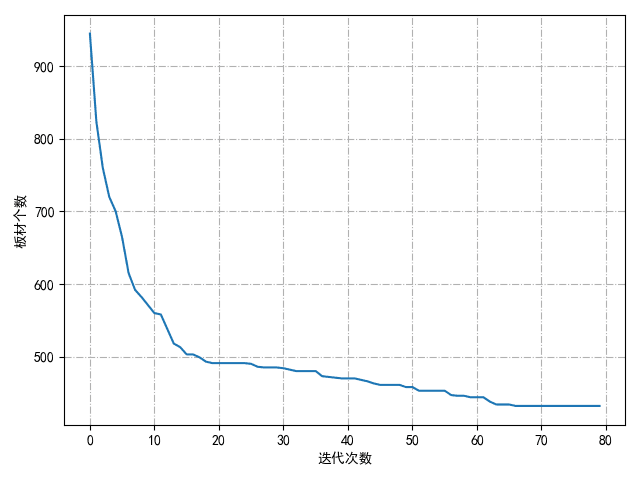
\includegraphics[width=.49\textwidth]{figures/d2.png}}\label{asdmd}
 	\subfigure[各方案生产产品数]{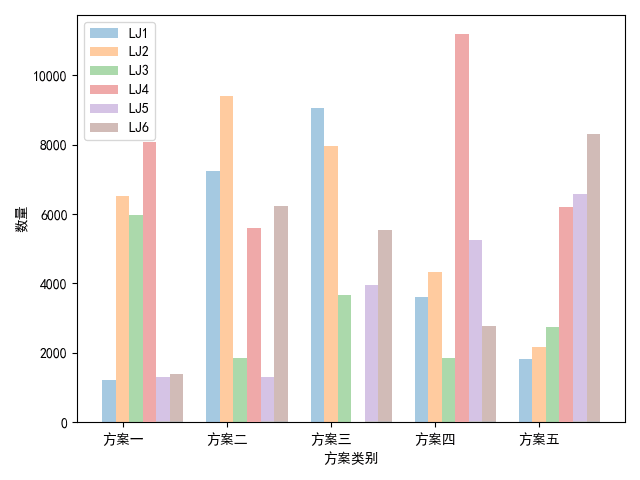
\includegraphics[width=.49\textwidth]{figures/f2.png}}
 	\caption{免疫差分进化算法结果图}\label{asddadamd}
 \end{figure}
 最优方案中各方案生产各类产品数如图~\ref{asddadamd}~(b)所示,其中方案一、方案二、方案三、方案四、方案五的生产细明如表
 \begin{table}[H]
 	\setstretch{}  %设置表的行间距
 	\centering		
 	\caption{问题三生产细明}\label{zhuanssssdasasgzai}
 	\begin{tabular}{cccccccc}
 		\toprule[2pt]
 		\multicolumn{1}{m{2cm}}{\centering }
 		& \multicolumn{1}{m{2cm}}{\centering 原材料数}
 		& \multicolumn{1}{m{1cm}}{\centering LJ1}
 		& \multicolumn{1}{m{1cm}}{\centering LJ2}
 		& \multicolumn{1}{m{1cm}}{\centering LJ3}
 		& \multicolumn{1}{m{1cm}}{\centering LJ4}
 		& \multicolumn{1}{m{1cm}}{\centering LJ5}
 		& \multicolumn{1}{m{1cm}}{\centering LJ6}
 		\\
 		\midrule[1pt]
 		方案一 & 12 &  14472     &  78132  &     71640   &    96912 &      15768    &   10632\\ 
 		方案二 & 0&  0   &  0 &      0 &     0 &     0    &       0\\ 
 		方案三 & 29& 262392   &   230753   &   106488    &       0   &   114318    &  160776\\ 
 		方案四&  113&   408834 &     490307 &     207468 &    1263114&      593928    &  313236\\ 
 		方案五 & 332 & 601584   &   754304  &    914328 &    2061720&     1816040 &    1997312\\ 
 		总计 &487 &  1287282  &   1553496  &   1199924   &  3421746   &  2540054   &  2481956\\ 
 		生产要求 &$\backslash$ & 1272000&1521000 &1161000 & 3229500&2434500 & 2421000\\ 
 		多余生产 &$\backslash$ &  15282    &   32496   &   38924     & 192246    &  105554    &   60956\\
 		冗余比例 &$\backslash$&  1.20\%   & 2.14\% &   3.35\%   & 4.95\% &  4.34\%   & 2.52\% \\ 
 		\bottomrule[2pt]	
 	\end{tabular}
 \end{table}
 由表可知,优化结果只使用$4$种分割方案,即切割方案二生产数为$0$,且所有工件的生产冗余比例皆小于5\%,在可容忍范围内。
  	
  	    \section{问题五模型的建立与求解}
  	\subsection{问题描述与分析}
  	
  	
  	
  	\subsection{模型的建立与求解}
  	问题五要求在原材料数量给定的情况下,给出总利润最大的五种切割方案。定义单产品理想收益为当所有原材料由$LJi(i=1,2,...,9)$产品填充且利用率达到$100\%$时产生的总收益$revenue_i$,即
  	\begin{gather}
	revenue_i=\frac{n_0\cdot v_0\cdot \eta }{v_i}u_i,
  	\end{gather}
  	其中,$n_0$和$v_0$分别代表原材料的数量和一个原材料的容积,$v_i$和$u_i$分别是产品$LJi$的体积和单个$LJi$的利润,$\eta=100\%$是理想的利用率。算得总收益如表~\ref{danchan}~所示:
  	
  	\begin{table}[H]
  		\setstretch{0.6}  %设置表的行间距
  		\centering		
  		\caption{单产品理想收益}\label{danchan}
  		\begin{tabular}{ccc}
  			\toprule[2pt]
  			\multicolumn{1}{m{2cm}}{\centering 产品类型}
  			& \multicolumn{1}{m{4cm}}{\centering 单产品理想收益}
  			& \multicolumn{1}{m{5cm}}{\centering 占最大值的比率}
  			\\
  			\midrule[1pt]
  			LJ1 &  166661966.3&92.9526\%\\ 
  			LJ2 &  179994923.6&100\%\\ 
  			LJ3 &  39446619.24&21.9154\%\\ 
  			LJ4 &  47561084.32&26.4236\%\\ 
  			LJ5 &  46279686.51&25.7117\%\\ 
  			LJ6 &  44377446.65&24.6548\%\\ 
  			LJ7 &  28728888.89&15.9609\%\\ 
  			LJ8 &  27270000&15.1504\%\\ 
  			LJ9 &  23745306.12&13.1922\%\\ 
  			\bottomrule[2pt]	
  		\end{tabular}
  	\end{table}
  	由表可知三种长方体收益相对于其他产品的收益较低,因此只考虑六种厚度相同的柱体排样。

  	总利润可以表示为
  	\begin{gather}
  	benefit=\sum_{i=1}^{6}n_i \cdot u_i-n_0\cdot u_0,
  	\end{gather}
	其中已知原材料的数量$n_0=100$,单价$u_0=120000$,$n_i$和$u_i(i=1,2,...,9)$分别代表零件$LJi$的加工数量和单价。

  	在问题二的基础上,考虑体积限制,对第$j(j=1,2,...,100)$块原材料,有
  	\begin{gather}
  	\sum_{i=1}^{6}n_{ij} \cdot v_i\leq v_0.
  	\end{gather}
  	
  	以二维视角和矩形原材料区域二值化考察图案排样方案。记产品图案为$R_i$,每个以$1mm$为步长的正方形像素点记为$r_k$,以矩形原材料区域左下顶点为原点,母层公共长轴方向为$x$轴,建立直角坐标系,母层像素中心点$q_k(x_k,y_k)$。对两个图案$R_i$和$R_m$,图案$R_i$的坐标已经确定且位于母层,$R_m$移动后记为$R_m'$。记图案$R_i$中心点为$M(x_m,y_m)$,为使$R_i$和$R_m$最大程度靠近且无重合,对$\forall r_k \in R_m$,有
  	\begin{gather}
  	\sum_{k=1}^{n_{rm}}d_{mk}\geq\sum_{k'=1}^{n_{rm}}d_{mk'},\\
  	s.t.\left\{\begin{matrix}
  	d_{mk}\geq r_i,k=1,2,...,n_rm,
  	\\ 
  	R_m=\bigcup_{k=1}^{n_{km}}r_k,
  	\end{matrix}\right.
  	\end{gather}
  	其中,$n_{rm}$是图案$R_m$的像素个数,$d_{mk}$是图案$R_i$中心点为$M(x_m,y_m)$到图案$R_i$像素中心点$q_k(x_k,y_k)$的欧式距离。
  	

  	\subsection{结果分析}
  	
  	可以算得不同切割方案的总利润如表\ref{sgzai}所示。
	\begin{table}[H]
		\setstretch{0.6}  %设置表的行间距
		\centering		
		\caption{不同切割方案的总利润}\label{sgzai}
		\begin{tabular}{ccc}
			\toprule[2pt]
			\multicolumn{1}{m{3cm}}{\centering 方案号}
			& \multicolumn{1}{m{4cm}}{\centering 组合方式}
			& \multicolumn{1}{m{4cm}}{\centering 总利润}\\
			\midrule[1pt]
			m1 &  LJ6、LJ6&27088800\\ 
			m2 &  LJ4、LJ4&29731200\\ 
			m3 &  LJ5、LJ5&28471200\\ 
			m4 &  LJ4、LJ5&28999200\\ 
			m5 &  LJ1、LJ1&132720000\\ 
			m6 &  LJ2、LJ2&144168000\\ 
			m7 &  LJ6、LJ2&75134400\\ 
			m8 &  LJ5、LJ6&27302400\\ 
			m9 &  LJ3、LJ3&22156800\\ 
			m10 &  LJ5、LJ2&73238400\\ 
			m11 &  LJ4、LJ6&27278400\\ 
			m12 &  LJ3、LJ1&50697600\\ 
			m13 &  LJ3、LJ2&49617600\\ 
			m14 &  LJ3、LJ6&22228800	\\ 
			m15 &  LJ4、LJ2&68580000\\ 
			m16 &  LJ3、LJ4&22929600\\ 
			m17 &  LJ3、LJ5&22305600\\ 
			m18 &  LJ1、LJ2&130104000\\ 
			\bottomrule[2pt]	
		\end{tabular}
	\end{table}
	可以看出,全为LJ2产品排样时候,总利润最大,为$144168000$元。
  	\section{灵敏度分析}
  	问题一中改变工具LJ1的基本参数长轴与短轴直径,使其上下波动 5\%,观察在固定贝叶斯优化后椭圆角度不变的情况下,利用率随椭圆长短轴直径变化是否发生改变。据图~\ref{adad}~分析可知,椭圆柱的长轴和短轴的变化对利用率的影响呈锯齿形状,说明在原料利用率是不稳定,会随着底面形状而发生改变。
  	
   \begin{figure}[H]
 	\centering
 	\subfigure{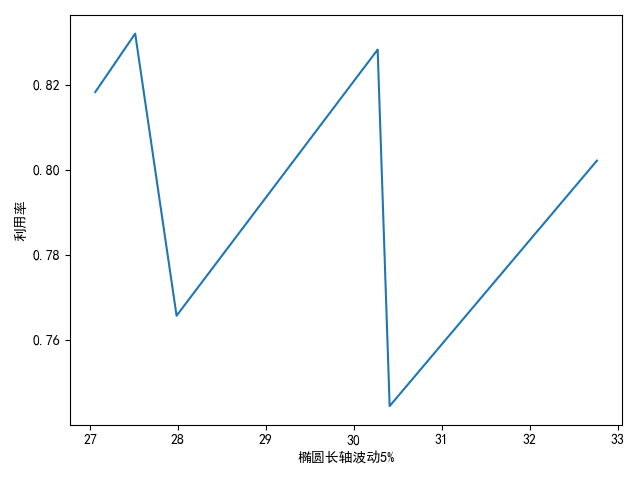
\includegraphics[width=.49\textwidth]{figures/lingmingdu/f3.png}}
 	\subfigure{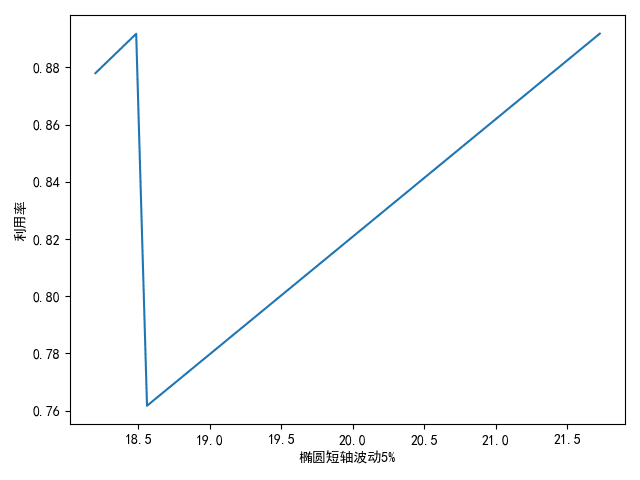
\includegraphics[width=.49\textwidth]{figures/lingmingdu/f4.png}}
 	\caption{工件LJ1长轴与短轴分别波动5\%}\label{adad}
 \end{figure}
   	
   	问题二中改变原材料的基本参数长度与宽度,使其上下波动 5\%,观察在固定在前五种利用率情况下,利用率随原材料改变是否发生改变。据图~\ref{adasfasad}~分析可知,原料的长宽发生改变时,五种方案利用率的排名也会有所变化,表明原料的大小也对工件生产利用率造成影响。
    \begin{figure}[H]
 	\centering
 	\subfigure{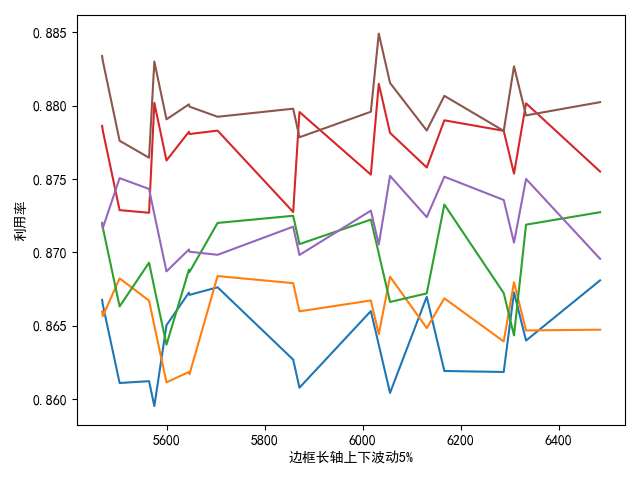
\includegraphics[width=.49\textwidth]{figures/lingmingdu/f1.png}}
 	\subfigure{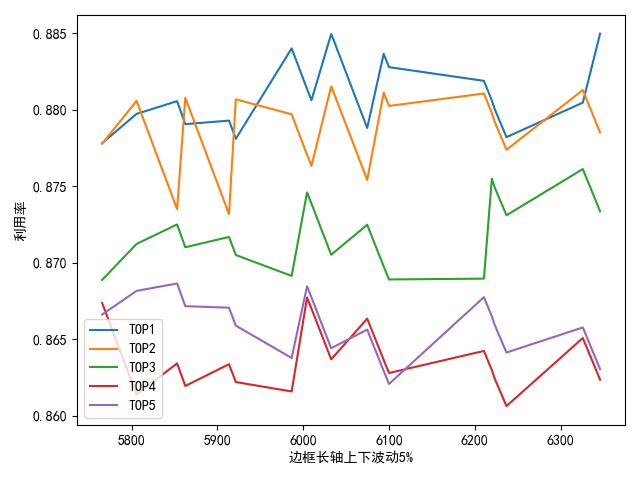
\includegraphics[width=.49\textwidth]{figures/lingmingdu/f2.png}}
 	\caption{原材料长度与宽度分别波动5\%}\label{adasfasad}
 \end{figure}
 
 
  	\section{模型的评价}
		\subsection{模型的优点}
			\begin{itemize}                                             
			\item [(1)]使用免疫差分进化优化切割比例,其运算速度较快,且有效防止算法陷入局部最优解,抑制算法早熟,兼顾了局部搜索与全局搜索能力。
			\item [(2)] 将三维排样问题转化为二维排样问题,并使用最小势能堆积算法有效降低了问题求解难度,大幅度降低了运算成本。
			\end{itemize}
		\subsection{模型的缺点}
		考虑到运算成本,未将所有种类产品同时进行三维排样,所得切割方案可能不是全局最优解。
  		\subsection{模型改进}

  
  
 
	\newpage	%换页符
	%%参考文献
	%\begin{thebibliography}{9}%宽度9
	% \setlength{\itemsep}{-2mm}
		\addcontentsline{toc}{section}{参考文献}
	\nocite{*}		%排版未引用的参考文献
	\begin{thebibliography}{9}%宽度9
		\bibitem{1}Pankratov A, Romanova T, Litvinchev I. Packing ellipses in an optimized rectangular container[J]. Wireless Networks, 2018: 1-11.
		\bibitem{2}Morales I P, Valera R R, Morfa C R, et al. Dense packing of general-shaped particles using a minimization technique[J]. Computational Particle Mechanics, 2017, 4(2): 165-179.
		\bibitem{3}郭晓雯, 杨鼎强. 在线约束性可变尺寸球体三维装箱[J]. 计算技术与自动化, 2019 (3): 18.
		\bibitem{4}李龙澍, 翁晴晴. 基于反向学习的自适应差分进化算法[J]. 计算机应用, 2018, 38(2): 399-404.
		\bibitem{5}Fernique T. A Densest ternary circle packing in the plane[J]. arXiv preprint arXiv:1912.02297, 2019.
		\bibitem{6}尚正阳, 顾寄南, 唐仕喜, 等. 高效求解三维装箱问题的剩余空间最优化算法[J]. 计算机工程与应用, 2019 (5): 7.
		\bibitem{8}Snoek J, Larochelle H, Adams R P. Practical bayesian optimization of machine learning algorithms[C]//Advances in neural information processing systems. 2012: 2951-2959.
	\end{thebibliography}

	\newpage
	%附录
	\appendix %%附录
	\section{仿真实验代码}
		\subsection*{问题一贝叶斯优化代码--python源代码}
		\lstinputlisting[language={python},numbers=left,numberstyle=\tiny,
		rulesepcolor=\color{red!20!green!20!blue!20},  
		keywordstyle=\color{blue!70!black},  
		commentstyle=\color{blue!90!},  
		basicstyle=\ttfamily] {./code/q1.py}

			
		\subsection*{第二问最小势能代码--python源代码}
		\lstinputlisting[language={python},numbers=left,numberstyle=\tiny,
	rulesepcolor=\color{red!20!green!20!blue!20},  
	keywordstyle=\color{blue!70!black},  
	commentstyle=\color{blue!90!},  
	basicstyle=\ttfamily] {./code/q2.py}
	
			\subsection*{第三问免疫差分进化代码--python源代码}
	\lstinputlisting[language={python},numbers=left,numberstyle=\tiny,
	rulesepcolor=\color{red!20!green!20!blue!20},  
	keywordstyle=\color{blue!70!black},  
	commentstyle=\color{blue!90!},  
	basicstyle=\ttfamily] {./code/q3.py}
	
	\subsection*{第四问三维装箱问题--python源代码}
	\lstinputlisting[language={python},numbers=left,numberstyle=\tiny,
		rulesepcolor=\color{red!20!green!20!blue!20},  
		keywordstyle=\color{blue!70!black},  
		commentstyle=\color{blue!90!},  
		basicstyle=\ttfamily] {./code/q4.py}
		
		\subsection*{第四问四种方式排列前6个工件--python源代码}
	\lstinputlisting[language={python},numbers=left,numberstyle=\tiny,
	rulesepcolor=\color{red!20!green!20!blue!20},  
	keywordstyle=\color{blue!70!black},  
	commentstyle=\color{blue!90!},  
	basicstyle=\ttfamily] {./code/q4t2.py}
	

\end{document}